\begin{ParaColumn}[\bisection*{Introduction}{介绍}]

    Owing to their massive production potential by quarrying and their mechanical properties in the dense state, rockfills are frequently used in civil engineering works. These granular fills are mainly composed of a mix of sand and angular rock aggregates with oversized particles that are too large to be handled by standard laboratory devices for compression and shearing. Alternative laboratory and in situ large direct shear tests have been developed by others \citep{Barton1981873,Matsuoka200192,Estaire200673}. However, these methodologies only allow for the evaluation of the mechanical behavior at low stresses, while calibration of new constitutive models that have been specifically developed for rockfill behavior \citep{Chávez2003215,Varadarajan2003206,Xiao20171,Yin2017} require accurate data on stress-strain controlled response over a large range of stresses. Therefore, a common challenge that engineers face when designing rockfill structures is that published information which documents large-scale tests is very scarce.

    \switchcolumn

    由于其巨大的采石生产潜力和致密状态下的机械性能,碎石经常用于土木工程。 这些颗粒状填充物主要由砂和角砾石骨料与超大颗粒的混合物组成,由于颗粒太大,无法通过标准实验室设备进行压缩和剪切处理。 有人已经开发了替代的实验室和现场大型直接剪切试验\citep{Barton1981873,Matsuoka200192,Estaire200673}。 但是,这些方法仅可用于评估低应力下的力学行为,而新的校准本构模型\citep{Chávez2003215,Varadarajan2003206,Xiao20171,Yin2017}是专门为碎石力学行为开发的,这需要在大范围的应力应变控制下的响应的准确数据。因此,工程师在设计碎石结构时面临的共同挑战是,记录大规模试验的公开信息非常稀缺。

    \switchcolumn*

    The largest triaxial testing apparatus ever built handles specimens with a diameter of ∼1 m. While equipment of this scale has been built, there are few examples currently in use due to the high cost involved in their maintenance and operation. Pioneering development of testing on very large samples was first reported during the 1960s at the laboratories of Karlsruhe Technical University \citep{Leussink1960}, the University of California at Berkeley (UCB) \citep{Marachi1969}, and the Federal Electricity Commission of Mexico (CFE) \citep{Marsal1965}. These groups designed and built devices that could handle samples ranging in diameter ($D$) from 914 to 1,130 mm, and having a maximum particle size (dmax) of 200 mm using the classic minimum aspect ratio $D/d_{\max}=$ 5 to 6 \citep{Holtz19561}. Experimental programs at CFE and UCB were carried out on several rockfill dam materials, and the results have become a reference for engineers and researchers. Part of the data produced at the CFE and UCB laboratories has been analyzed in detail and used to propose empirical correlations and ranges for mechanical parameters of coarse rockfill materials \citep{Leps19701159,Barton1981873,Hunter2003909}. Other authors have subsequently reported new results and have updated the database \citep{Charles1980353,Al-Hussaini1983706,Matsuoka1998275,Hunter2003909,Varadarajan2003206,Xiao2014a,Xiao2014b} using triaxial cells that can take samples of 300–500 mm in diameter. These studies have significantly advanced the understanding of the mechanical behavior of rockfills, such as the study of the effects of partial saturation \citep{Oldecop2003289,Alonso2016455}, stress path \citep{Chávez2003215,Xiao2016}, and particle size \citep{Verdugo2007243,Hu2011,Ovalle20201}.

    \switchcolumn

    历史上最大的三轴试验设备可处理直径约1米的样本。 虽然这种规模的设备已经可以制造,但是由于维护和操作成本高昂,目前很少使用这些设备。  1960年代,卡尔斯鲁厄技术大学\citep{Leussink1960},加利福尼亚大学伯克利分校(UCB)\citep{Marachi1969}和墨西哥联邦电力委员会的实验室(CFE)\citep{Marsal1965}首次报道了对大型样品进行试验的开创性发展。这些小组设计和制造了可以处理直径($D$)从914到1130毫米范围的样品,并且使用经典的最小长宽比$D/d_{\max}=5\sim 6$ \citep{Holtz19561}。 CFE和UCB的试验程序是在几种碎石坝材料上进行的,其结果已成为工程师和研究人员的参考。 许多人对CFE和UCB实验室得到的部分数据进行了详细分析,并用于提出经验性的相关性和取值范围范围,用作粗碎石料的力学参数\citep{Leps19701159,Barton1981873,Hunter2003909}。 其他作者随后使用可以采集直径为300-500毫米的土体样品的三轴试验报告了新的结果并更新了数据库\citep{Charles1980353,Al-Hussaini1983706,Matsuoka1998275,Hunter2003909,Varadarajan2003206,Xiao2014a,Xiao2014b}。 这些研究极大地促进了对碎石力学行为的理解,例如对部分饱和度的影响\citep{Oldecop2003289,Alonso2016455},对应力路径\citep{Chávez2003215,Xiao2016}和对颗粒粒径\citep{Verdugo2007243,Hu2011,Ovalle20201}的研究。

    \switchcolumn*

    Due to the size limitation of testing devices, a common practice is to test small-scale samples with a parallel gradation while maintaining the particle shape, mineralogy, and sample aspect ratio. However, it has been proven that this method may be limited due to size effects on particle crushing \citep{Marachi1969,Frossard2012415,Ovalle20142199}. \enautoref{figure:1} presents the results of several diametral compressions of individual rock aggregates between two stiff parallel platens where crushing strength decreases when particle size increases, which is consistent with the brittle fracture mechanics theory \citep{Weibull19391}. Therefore, the amount of particle crushing is less in small-scale (i.e., finer) granular materials than in coarser prototype materials.

    \switchcolumn

    由于试验设备的尺寸限制,通常的做法是在保持颗粒形状,矿物质和样品长宽比不变的同时,对小尺度样品进行平行试验。 但是,已经有人证明该方法可能会由于尺寸上的影响而受到限制\citep{Marachi1969,Frossard2012415,Ovalle20142199}。 \cnautoref{figure:1}给出了两个刚性平行压板之间单个岩石聚集体的多次径向压缩的结果,其中,当粒径增大时,抗压强度降低,这与脆性断裂力学理论\citep{Weibull19391}一致。 因此,小颗粒物料的颗粒破碎量比粗颗粒物料的颗粒破碎量要小。

    \CrossColumnText{
        \begin{figure}[htb]
    \centering
    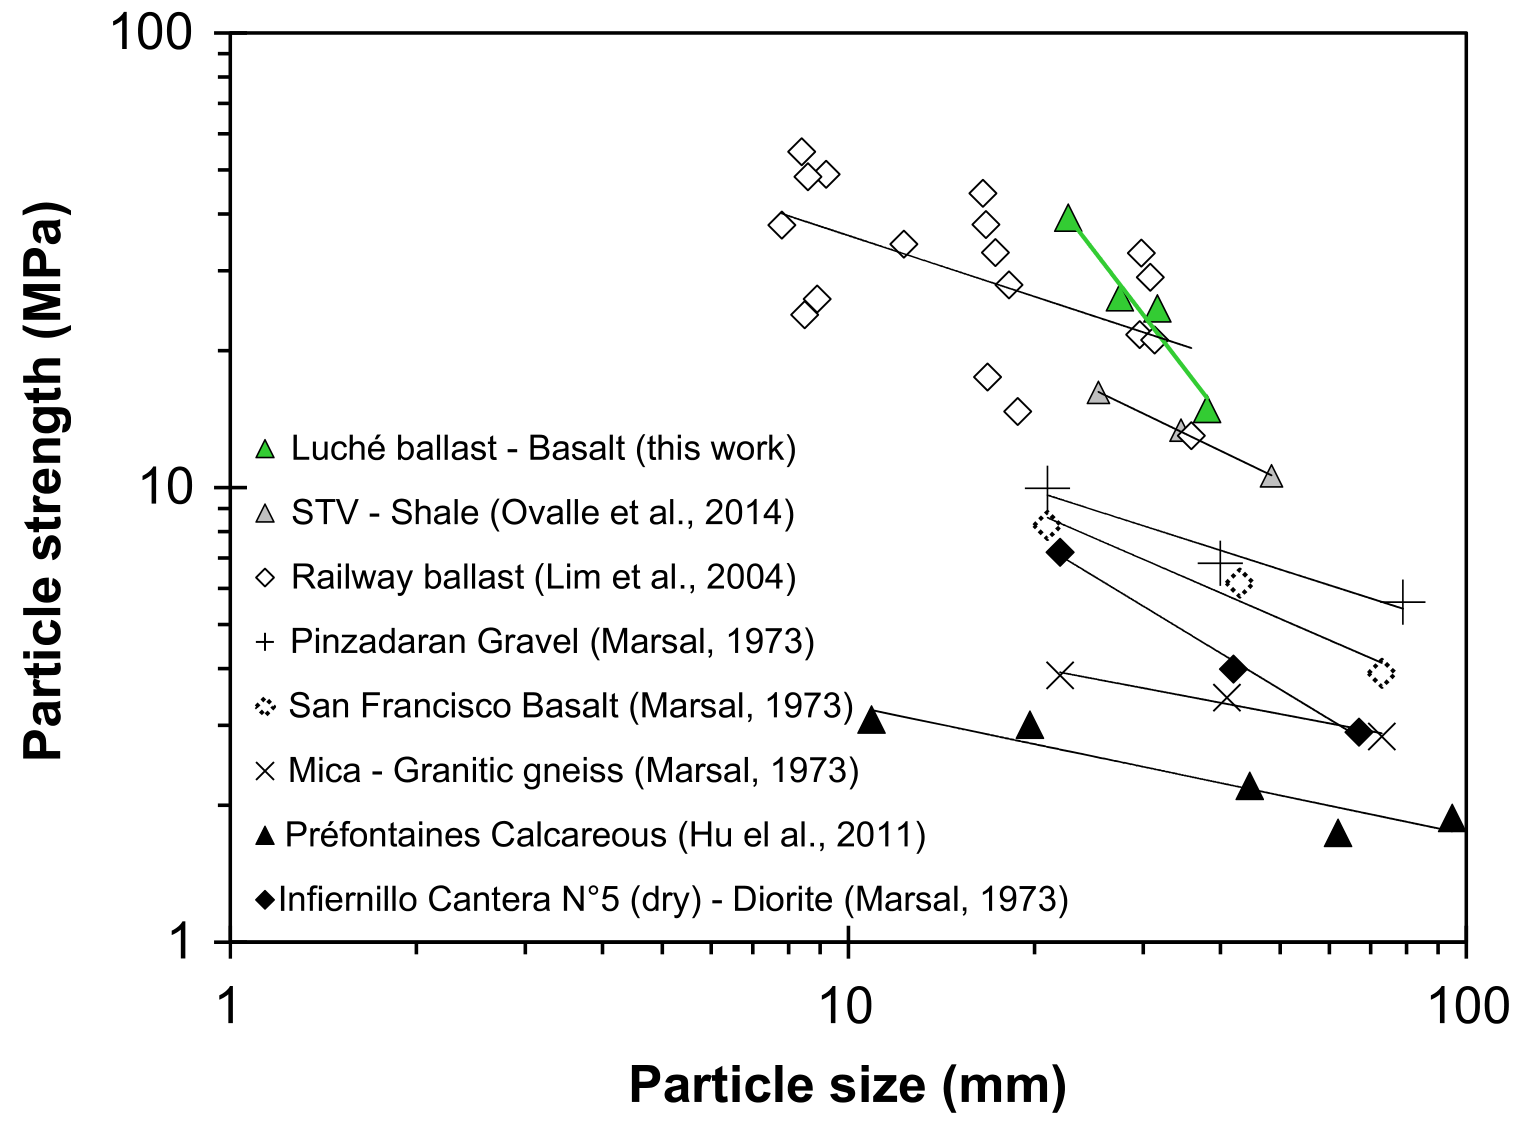
\includegraphics[width=0.5\textwidth]{figures/figure-1.png}
    \bicaption{Particle crushing strength of rock aggregates}{骨料的颗粒破碎强度}
    \label{figure:1}
\end{figure}
    }

    \switchcolumn*

    Along with presenting new tests carried out in recent, very large triaxial devices, the aim of this study was to consolidate and extend the existing database through the compilation of data on large triaxial tests on coarse rockfill samples carried out between the 1960s and the 2000s. To present comparable results in terms of stress path, particle size, and particle shape, only drained compression triaxial tests on coarse rockfills samples of $\sim 1$ m in diameter, composed of angular shaped grains with $d_{\max}$ between 100 and 200 mm, have been considered. Results from 158 tests on samples from 33 rockfill materials are presented. The influence of the confining stress and the amount of particle crushing on shear strength and secant stiffness is discussed. To highlight the data on coarse crushable rockfill materials, the results were compared with published data on finer materials, such as dense uniform quartzitic sands and railway ballasts.

    \switchcolumn

    除了介绍最近在非常大的三轴设备中进行的新试验外,本研究的目的是通过汇编有关在1960年代至2000年代之间进行的粗碎石料样品的大型三轴试验的数据来加强和扩展现有数据库。 为了在应力路径,粒度和颗粒形状方面提供可比的结果,仅考虑了对直径约1米的粗碎石样品进行的排水三轴试验,该样品由$d_{\max}$在100至200毫米之间的角状晶粒组成。 给出了158种试验结果,这些结果来自33种碎石材料的样品。 讨论了围压和颗粒破碎量对剪切强度和割线刚度的影响。 为了突出有关粗碎石料的数据,将结果与已发布的有关较细材料的数据进行了比较,如致密均匀的石英砂和铁道石渣。

\end{ParaColumn}